%\RequirePackage{lineno}
%\documentclass[aps,prl,twocolumn,showpacs,groupedaddress]{revtex4}  % for review and submission
%\usepackage{graphicx}  % needed for figures
%\usepackage{dcolumn}   % needed for some tables
%\usepackage{bm}        % for math
%\usepackage{amssymb}   % for math

%\usepackage{url}
%\usepackage{appendix}
%\usepackage{setspace}
%\usepackage{xspace}
%\usepackage{verbatim}
%\usepackage{color}
%\usepackage{lineno}


% Customizable fields and text areas start with % >> below.
% Lines starting with the comment character (%) are normally removed before release outside the collaboration, but not those comments ending lines

% svn info. These are modified by svn at checkout time.
% The last version of these macros found before the maketitle will be the one on the front page,
% so only the main file is tracked.
% Do not edit by hand!
\RCS$Revision: 153561 $
\RCS$HeadURL: svn+ssh://svn.cern.ch/reps/tdr2/papers/SMP-12-004/trunk/SMP-12-004.tex $
\RCS$Id: SMP-12-004.tex 153561 2012-10-18 16:05:03Z gaultney $
%%%%%%%%%%%%% local definitions %%%%%%%%%%%%%%%%%%%%%
% This allows for switching between one column and two column (cms@external) layouts
% The widths should  be modified for your particular figures. You'll need additional copies if you have more than one standard figure size.
\newlength\cmsFigWidth
\ifthenelse{\boolean{cms@external}}{\setlength\cmsFigWidth{0.85\columnwidth}}{\setlength\cmsFigWidth{0.4\textwidth}}
\ifthenelse{\boolean{cms@external}}{\providecommand{\cmsLeft}{top}}{\providecommand{\cmsLeft}{left}}
\ifthenelse{\boolean{cms@external}}{\providecommand{\cmsRight}{bottom}}{\providecommand{\cmsRight}{right}}
%%%%%%%%%%%%  Title page %%%%%%%%%%%%%%%%%%%%%%%%
\cmsNoteHeader{SMP-14-Vbb} % This is over-written in the CMS environment: useful as preprint no. for export versions
% >> Title: please make sure that the non-TeX equivalent is in PDFTitle below
%\title{Measurement of Z/gamma + jet angular distributions}

%\begin{document}
%\setpagewiselinenumbers
%\modulolinenumbers[5]
%\linenumbers

\title{Production of a W or Z boson in association with b quarks in proton-proton collisions at 8 TeV}


% >> Authors
%Author is always "The CMS Collaboration" for PAS and papers, so author, etc, below will be ignored in those cases
%For multiple affiliations, create an address entry for the combination
%To mark authors as primary, use the \author* form
\address[Wisconsin]{Wisconsin}
\address[Trieste]{Trieste}
\address[cern]{CERN}
\address[Zagreb]{Zagreb}
\author[cern]{The CMS Collaboration}

% >> Date
% The date is in yyyy/mm/dd format. Today has been
% redefined to match, but if the date needs to be fixed, please write it in this fashion.
% For papers and PAS, \today is taken as the date the head file (this one) was last modified according to svn: see the RCS Id string above.
% For the final version it is best to "touch" the head file to make sure it has the latest date.
\date{\today}

% >> Abstract
% Abstract processing:
% 1. **DO NOT use \include or \input** to include the abstract: our abstract extractor will not search through other files than this one.
% 2. **DO NOT use %**                  to comment out sections of the abstract: the extractor will still grab those lines (and they won't be comments any longer!).
% 3. **DO NOT use tex macros**         in the abstract: External TeX parsers used on the abstract don't understand them.
\abstract{
The production of a vector boson (W or Z) in association with one or more b jet is studied using proton-proton collisions recorded by the CMS detector at the LHC center-of-mass energy of 8 TeV. This assumes the decay mode $Z/\gamma^* \to \ell^+ \ell^-$ and  $W^\pm\to \ell^\pm \nu$, where $\ell=\rm{e}$ or $\mu$. Beside the inclusive production cross-section estimation, several key quantities are unfolded from detector effect and compared with predictions from theory, at tree-level and NLO accuracy. Besides, an estimation of the cross-section corresponding to the case where 2 b-hadrons are inside a single jet is performed.This study provides a strong test of the QCD predictions and gets further in understanding  the 
dynamics of heavy quark production in association with vector bosons.
}

%\end{abstract}

% >> PDF Metadata
% Do not comment out the following hypersetup lines (metadata). They will disappear in NODRAFT mode and are needed by CDS.
% Also: make sure that the values of the metadata items are sensible and are in plain text (no TeX! -- for \sqrt{s} use sqrt(s) -- this will show with extra quote marks in the draft version but is okay).

\hypersetup{
pdfauthor={A.-M. Magnan, S. de Visscher},
pdftitle={Production of a vector boson (W or Z) in association with one or more b quarks in proton-proton collisions at 8 TeV},
pdfsubject={CMS},
pdfkeywords={CMS, physics, Z boson, W boson, B hadrons, b jets, angular distribution, QCD, perturbative test}
}

\maketitle 
%maketitle comes after all the front information has been supplied

%%%%%%%%%%%%%%%%%%%%%%%%%%%%%%%%%%%%%%%%%%%%%%%%%%

\section{Introduction}
\label{sec:intro}

The measurement of \cPZ$/\cPgg^*$ (henceforth denoted by ``\cPZ'') or
\Wpm production in association with b quarks in proton-proton
collisions at the Large Hadron Collider (LHC) is relevant for various
experimental searches. In particular, these processes constitute a
background to standard model (SM) Higgs production associated with a
\cPZ~or a \Wpm boson, where the Higgs boson decays into a $b\bar{b}$
pair. The discovery by the ATLAS and Compact Muon Solenoid (CMS)
experiments of a neutral boson with a mass of about
$125\GeV$~\cite{Aad20121,:2012gu} motivates further studies to
establish its nature and determine the coupling of the new boson to b
quarks. Furthermore, different models based on an extension (minimal
or not) of the Higgs sector are being tested against the LHC data
through final states composed of lepton(s) and b-jet(s).  In this
context, a better understanding of the b-hadrons and/or associated
jets dynamics, as well as of the vector boson is required to refine
the background prediction and increase the sensitivity to new physics.

In addition, the study of the angular correlations for the collinear
production of b quarks, where large theoretical uncertainties remain
[ref?]  provides a strong lever arm on predictions from
theory. Tree-level calculations allowing for large numbers of extra
partons in the matrix elements (as initial- and final-state
radiations) are available. These are provided by
\MADGRAPH~\cite{Alwall:2007st,Alwall:2011uj}, 
{\ALPGEN~\cite{alpgen}, and \SHERPA~\cite{Gleisberg:2008ta},
in both the five- and four-flavour approaches, \ie by considering the
five or four lightest quark flavours in the proton parton distribution
function (PDF) sets. Next-to-leading-order (NLO) calculations have
been performed in both the five-flavour (\MCFM)~\cite{Campbell:2000bg}
and four-flavour~\cite{FebresCordero:2008ci,Cordero:2009kv}
approaches. A fully-automated NLO computation matched to a parton
shower simulation is implemented by the a\MCATNLO event
generator~\cite{Frederix:2011qg,Frixione:2002ik}. A detailed
discussion of b-quark production in the different calculation schemes
is available in Ref.~\cite{Maltoni:2012pa}.

From the experimental point of view, final states containing one or
two leptons (electrons or muons) and one ore more b-flavoured objects
are selected. Leptons from the vector-boson decays are expected to be
energetic and isolated, which provide a clean way of selecting the
events at the trigger level. The study of b-flavoured final states is
possible through two complementary techniques. First using the
standard jet-based b-tagging methods~\cite{Chatrchyan:2012jua}. These
techniques are dominantly considered in searches sensitive to the
emission of b jets. Second via the complementary approach that
identifies the b hadrons from displaced secondary vertices, which are
reconstructed from their charged decay products. This approach is
implemented in the inclusive secondary vertex finder
(IVF)~\cite{Khachatryan:2011wq}. The IVF exploits the excellent
tracking capabilities of the CMS detector and, being independent of
the jet reconstruction, extends the sensitivity to small angular
separations and softer b-hadron transverse momenta ($\pt$). Background
processes are mainly top processes (\ttbar and single top),
misidentification of light or charm-flavoured objects, dibosons, and
multijet production for the case of the \Wpm\ bosons.
 
In the past, the production of \cPZ+1 and 2 b
jets~\cite{Chatrchyan:2012vr,Chatrchyan:2014dha,Chatrchyan:2013zja,Aad:2011jn,Aad:2014dvb},
and \Wpm+ b jets~\cite{Chatrchyan:2013uza,Aad:2013vka} have been
studied by the ATLAS and CMS collaborations, at a centre-of-mass
energy $\sqrt{s}$ of 7 TeV using up to 5~fb$^{-1}$ of integrated
luminosity.

This article presents several studies. First, precise measurements,
not statistically limited, of the unbinned production cross section
for \cPZ+1 and 2 b-jets, and \Wpm+2 b-jets, are re-iterated at
$\sqrt{s}=8$ TeV. This is particularly important for the comparison
with the normalisation predictions provided at NLO.

Second, differential production cross sections are measured as a
function of several variables: $\pt^{\rm V}$ where V=\cPZ, \Wpm,
$\pt^{\cPqb_i}$ and $\eta^{\cPqb_i}$ where $i$ is denoting the list of
b jets sorted by transverse momentum, the mass of the b-jets system
$m^{\cPqb_1,\cPqb_2}$. These variables are considered in searches for
new physics states through channels involving b jets, and a comparison
between the data and predictions from theory is therefore crucial to
understand how well the predicted shapes match the reality.

Third, the production cross section of the processes where two b
hadrons are found in one single jet is provided, as well as the
angular correlations between the two b hadrons: $\Delta
R_{\mathrm{BB}}$ and $\Delta\phi_{\mathrm{BB}}$. The variable $\Delta
R_{\mathrm{BB}}$ is defined as $\Delta R_{\mathrm{BB}} = \sqrt{
  (\Delta \phi_{\mathrm{BB}})^2 + (\Delta \eta_{\mathrm{BB}})^2}$,
where $\Delta \phi_{\mathrm{BB}}$ and $\Delta \eta_{\mathrm{BB}}$ are
the azimuthal (in radians) and pseudorapidity separations. The
pseudorapidity is defined as $\eta= -\ln[\tan(\theta/2)]$, where
$\theta$ is the polar angle relative to the anticlockwise beam
direction. Besides helping to understand the contamination of V+2 b
hadrons inside one jet to V+1 b hadron in one jet, the $\Delta
R_{\mathrm{BB}}$ distribution constitutes a direct test of the
modeling of the different $\mathrm{pp}\rightarrow {\rm V}
\bbbar\mathrm{X}$ production modes. This quantity allows the
identification of the contribution from the $\cPq{i} \rightarrow {\rm
  V} \bbbar \mathrm{X}$ subprocesses (where $i=\cPq$, $\cPg$) for
which the scattering amplitude modelling is based on Feynman diagrams
with a final $\cPg \rightarrow \bbbar$ splitting. In particular, at
leading order, and assuming no selection on the transverse momentum of
the vector boson, this type of subprocess is dominant over the whole
$\Delta R_{\mathrm{BB}}$ range for $\Wpm b\overline{b}$ while it is
true only for small $\Delta R_{\mathrm{BB}}$ for $\cPZ b\overline{b}$
process. This is due to the dominant subprocesses with two
initial-state gluon splittings or where the \cPZ\ is radiated off a
final-state b-quark line. In these cases, the angular correlation
between the b quarks is much weaker. A leading-order diagram for both
$\cPq\cPq\rightarrow \cPZ b\overline{b}$ and $\cPq\cPq\rightarrow \Wpm
b\overline{b}$ is shown in Fig.~\ref{diag} (a), together with
diagrams representative of other $\mathrm{pp}\rightarrow\cPZ\bbbar$
production modes: emission of a \cPZ~boson from a b-quark line (b),
and b-quark fusion $\cPg\cPg \rightarrow \cPZ\bbbar$ (c).

\begin{figure}[!t]
	\begin{center}
	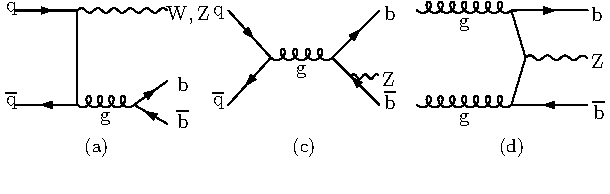
\includegraphics[width=0.5\textwidth]{figures_for_paper/croppedWZbb.pdf}
	\caption{Tree-level Feynman diagrams for (a) $\cPq\cPq
          \rightarrow {\rm V}\bbbar$ subprocess
          involving $\cPg\rightarrow \bbbar$
          splitting; (b)  $\cPq\cPaq \rightarrow \cPZ\bbbar$ with the
          emission of a $ \cPZ$~boson from a b quark; and (c) $\cPg\cPg \rightarrow \cPZ\bbbar$.}
\label{diag}	
	\end{center}
\end{figure}

For each measurement, the observed results are compared to several
theoretical predictions.


The sections are organized as follows: the description of the CMS
experiment is given in Section~\ref{sec:cms}; data and Monte-Carlo
samples are detailed in Section~\ref{sec:samples}; the objects
reconstruction and selection are presented in
Section~\ref{sec:eventrecoandselection}. The discussions on the
inclusive and differential cross-section measurements (based on b
jets) are found in Section~\ref{sec:bjetinclusivexsec} and
Section~\ref{sec:bjetdifferentialxsec}.  The measurement of the cross
section corresponding to the collinear production of b hadrons and the
discussion on angular correlation between the b hadrons are detailed
in Section~\ref{sec:collxsec}. The conclusions are presented in
Section~\ref{sec:conclusions}.


\section{CMS detector}
\label{sec:cms}


The central feature of the CMS apparatus is a superconducting solenoid
of 6\unit{m} internal diameter, providing a magnetic field of
3.8\unit{T}. Within the superconducting solenoid volume are a silicon
pixel and strip tracker, a lead tungstate crystal electromagnetic
calorimeter (ECAL), and a brass/scintillator hadron calorimeter
(HCAL), each composed of a barrel and two endcap sections. Muons are
measured in gas-ionization detectors embedded in the steel flux-return
yoke outside the solenoid. Extensive forward calorimetry complements
the coverage provided by the barrel and endcap detectors.

The most relevant detector element for the identification of b jets is
the tracking system. The inner tracker consists of 1440 silicon pixel
and 15 148 silicon strip detector modules. It measures charged
particles up to a pseudorapidity of $|\eta| < 2.5$. The pixel modules
are arranged in three cylindrical layers in the central part of CMS
and two endcap disks on each side of the interaction point. The sili-
con strip detector comprises two cylindrical barrel detectors with a
total of 10 layers and two endcap systems with a total of 12 layers at
each end of CMS. The tracking system provides an impact parameter (IP)
resolution of about 15 $\mu$m at a \pt of 100 GeV. In comparison
typical IP values for tracks from b-hadron decays are at the level of
a few 100 $\mu$m. 

Muons are measured and identified in detection layers that use three
technologies: drift tubes, cathode-strip chambers, and resistive-plate
chambers. The muon system covers the pseudorapidity range $|\eta| <
2.4$. The combination of the muon and tracking systems yields muon
candidates of high purity with a \pt resolution between 1 and 5\%, for
\pt values up to 1 TeV. The ECAL energy resolution for electrons with
$\ET {\approx} 45$\GeV from $\Z \rightarrow \Pe \Pe$ decays is better
than 2\% in the central region of the ECAL barrel $(\abs{\eta} <
0.8)$, and is between 2\% and 5\% elsewhere. For low-bremsstrahlung
electrons, where 94\% or more of their energy is contained within a $3
\times 3$ array of crystals, the energy resolution improves to 1.5\%
for $\abs{\eta} < 0.8$~\cite{Chatrchyan:2013dga}.

A more detailed description of the CMS detector, together with a
definition of the coordinate system used and the relevant kinematic
variables, can be found in Ref.~\cite{Chatrchyan:2008zzk}.

\section{Data and Monte-Carlo samples}
\label{sec:samples}

The data were taken in 2012. Beam conditions changed during the year
in order to provide the highest instantaneous luminosity possible,
which meant that the average number of secondary minimum bias
interactions (pileup) varied from about 10 to 35. Only luminosity
sections for which all subdetectors were fully operational are
considered for analysis. The total analysed integrated luminosity
amounts to $19.8 \pm 0.5$\,fb$^{-1}$~\cite{CMS-PAS-LUM-13-001}.

Events were triggered by single lepton (W) and dilepton triggers,
choosing the loosest unprescaled versions available. All triggers used
here are selecting leptons above given p$_T$ thresholds and passing
loose quality and isolation criteria. The single electron (muon)
trigger has a p$_T$ threshold on the electron (muon) of 27
(24)\,GeV). The single muon trigger also has a requirement on the
pseudorapidity $|\eta|<2.1$. The dielectron and dimuon triggers have
p$_T$ thresholds of 17 and 8\,GeV on the leading and subleading
leptons.

For \ttbar, W+jets and Z+jets processes, the Monte Carlo (MC)
simulation of events is done using the \madgraph
v5~\cite{Alwall:2011uj} matrix-element (ME) generator interfaced with
\pythia v6.4~\cite{Sjostrand:2006za} for the parton shower (PS), using
the Z2 tune~\cite{Khachatryan:2010nk}. Events are generated with up to
4 partons at tree-level. The different parton multiplicities are
merged into a single sample. The cteq6l1 PDF set is
used~\cite{Pumplin:2002vw}. Normalisation and factorisation scales are
set to XXX. The k$_T$-MLM ME-PS matching mechanism is used with a
scale set to 20 GeV. V+jets (\ttbar) samples are normalised to
inclusive NNLO cross sections obtained with FEWZ~\cite{Gavin:2010az} (

For single top processes, ...

Diboson events (WW, WZ and ZZ) are generated using ...

Alternative MC are considered in order to extract model uncertainties
(see Section~\ref{sec:syst})....

\section{Event reconstruction and selection}
\label{sec:eventrecoandselection}

\section{Inclusive cross-sections}
\label{sec:bjetinclusivexsec}

\section{Differential cross-section}
\label{sec:bjetdifferentialxsec}

\section{Collinear production cross-section of b-hadrons and related angular correlation}
\label{sec:collxsec}

\section{Conclusion}
\label{sec:concl}


%%%%%%%%%%%%%%%%%%%%%%%%%%%%%%%%%%%%%%%%%%%%%%%%%%


%\clearpage

%\end{document}


\bibliography{auto_generated} 
%\bibliographystyle{abbrv}
%\bibliography{SMP-12-004prl}

%\end{document}
